\documentclass[conference]{IEEEtran}
\IEEEoverridecommandlockouts
% The preceding line is only needed to identify funding in the first footnote. If that is unneeded, please comment it out.
\usepackage{cite}
\usepackage{amsmath,amssymb,amsfonts}
\usepackage{algorithmic}
\usepackage{algorithm}
\usepackage{graphicx}
\usepackage{textcomp}
\usepackage{xcolor}
\usepackage{float}

\def\BibTeX{{\rm B\kern-.05em{\sc i\kern-.025em b}\kern-.08em
    T\kern-.1667em\lower.7ex\hbox{E}\kern-.125emX}}
\usepackage{tikz}
\usetikzlibrary{arrows.meta,positioning}
\usepackage{pgfplots}
\pgfplotsset{compat=1.18}
\begin{document}

\title{Ant Colony Optimization Based Shortest Path Finding Algorithm\\
{\footnotesize \textsuperscript{}}
\thanks{}
}

\author{\IEEEauthorblockN{Vaibhav Verma}
\IEEEauthorblockA{\textit{Department of Computing Technologies} \\
\textit{SRM Institute Of Science and Technology}\\
Chennai, India \\
vv4834@srmist.edu.in}
\and

\IEEEauthorblockN{Kapish}
\IEEEauthorblockA{\textit{Department of Computing Technologies} \\
\textit{SRM Institute Of Science and Technology}\\
Chennai, India \\
ks4225@srmist.edu.in}
}


\maketitle

\begin{abstract}
The problem of finding the shortest path between two points is a fundamental problem in computer science and has wide applications in transportation, communication networks, robotics and route planning. This is a common task in many applications and algorithms such as Dijkstra’s algorithm and the A* algorithm are often used for this but they may become less flexible if the search space is large, complex or continuously changing. One such nature-inspired approach to optimization problems is Ant Colony Optimization (ACO).

The ACO is based on the real ant behavior in search of food. Ants communicate indirectly by laying down trails of pheromones on the paths they take. The greater the amount of pheromone, the more likely another ant will choose that route. Over time, the colony will find more efficient and shorter routes. In the computational version of this process artificial ants explore different possible paths and update the pheromone values based on the quality of the solutions found.

This background study is related to working principles of Ant Colony Optimization and its use for shortest path problem. It discusses important concepts like pheromone updating, heuristic information, path selection probability, evaporation rate and convergence. The benefits and limitations of ACO compared with the conventional shortest-path algorithms are also discussed in the research. The main objective is to understand the use of swarm intelligence in route optimization and the effectiveness of ACO in a dynamic and complex network environment.


\end{abstract}

\begin{IEEEkeywords}
Ant Colony Optimization, Shortest-Path Problem, Swarm Intelligence, Path Optimization, Bio-inspired Algorithms
\end{IEEEkeywords}


\section{INTRODUCTION}

One of the most fundamental problems in computer science is the shortest path optimization problem, which has important applications in transportation systems, communication networks, robotics, logistics and route planning. The main objective of this problem is to find the best path between two points minimizing distance, cost or time. Dijkstra’s algorithm and the A* algorithm are widely used to solve shortest path problems and provide optimal solutions in static environments. However, these approaches may not be appropriate for large-scale, dynamic and complex networks where the search space is changing frequently and requires adaptive optimization techniques.

Ant Colony Optimization (ACO) is a nature inspired metaheuristic optimization technique that was proposed by Dorigo et al. based on the foraging behavior of real ant colonies. While foraging for food, ants indirectly communicate by laying down pheromone trails on paths. The paths with higher pheromone concentration are more likely to be selected and the colony can gradually find shorter and more efficient paths. This behavior is used in artificial ants in computational systems to explore possible solutions, update pheromone information and improve the quality of paths over multiple iterations \cite{dorigo1996}.

ACO has been widely used to solve complex optimization and routing problems because of its flexibility and distributed search capability. Improvements such as Ant Colony System (ACS) proposed better pheromone updating and path selection strategies, improving convergence and solution quality compared to the original Ant System \cite{dorigo1997}. Furthermore, ACO-based shortest path approaches have been explored in dynamic routing environments, where network conditions are continuously changing, highlighting the effectiveness of swarm intelligence techniques for adaptive path optimization \cite{shortestpathaco}. In this paper, the working principles of ACO, such as pheromone initialization, heuristic information, transition probability, evaporation rate and convergence behavior are understood. At the same time, the advantages and limitations of ACO compared with conventional shortest path algorithms are analyzed.





\section{Literature Review}

Li et al. proposed an Intelligently Enhanced Ant Colony Optimization algorithm for mobile robot path planning. The method improved pheromone initialization and heuristic information to achieve faster convergence and better path quality \cite{ieaco2025}.

Ma et al. introduced an Improved Trimming Ant Colony Optimization algorithm for mobile robot path planning. Their approach reduced unnecessary path nodes using trimming strategies and improved the efficiency of generated paths \cite{itaco2025}.

Li et al. proposed a multi-strategy improved Ant Colony Optimization algorithm for robot path planning. The approach combined adaptive pheromone updating and optimization strategies to reduce premature convergence and improve search performance \cite{msgaco2025}.

Li et al. developed an improved Q-evaluation Ant Colony Optimization algorithm for mobile robot path planning. Their method enhanced node evaluation and improved path search stability compared with traditional ACO methods \cite{iqaco2025}.

Huang et al. proposed an improved ACO-based path planning approach for delivery robots. The study focused on improving obstacle avoidance, reducing search limitations and generating efficient navigation paths \cite{deliveryaco2025}.

Shi et al. presented an improved Ant Colony Optimization approach for mobile robot path planning. Their work enhanced path optimization by modifying heuristic functions and pheromone update mechanisms \cite{robotaco2025}.

Cui et al. proposed a multi-strategy adaptable Ant Colony Optimization algorithm for path planning. Their approach improved adaptability by dynamically adjusting optimization parameters during the search process \cite{adaptiveaco2025}.

Zhuo et al. proposed a multi-strategy enhanced Ant Colony Optimization algorithm for mobile robot path planning. The method improved pheromone initialization, state transition probability and pheromone updating strategies to overcome local optimum problems \cite{mseaco2026}.

Yu et al. proposed an enhanced Ant Colony Optimization algorithm for mobile robot path planning. The method improved convergence speed and path quality through optimized heuristic information and pheromone strategies \cite{enhancedaco2026}.

Liu et al. introduced the Pheromone-Focused Ant Colony Optimization algorithm for path planning. Their approach improved pheromone distribution to reduce redundant exploration and enhance optimization performance \cite{pfaco2026}.

Zeng et al. proposed a double-layer Ant Colony Optimization algorithm for robot navigation path planning. Their approach introduced improved scheduling mechanisms and angle constraints to generate stable and efficient paths \cite{idlaco2026}.

Recent studies demonstrate that Ant Colony Optimization provides an effective approach for shortest path and routing problems. However, challenges such as convergence speed, parameter tuning and adaptation to highly dynamic environments still require further research.


\section{Problem Description}

The shortest path problem is the problem of finding the most efficient route between a source and destination node in a given network minimizing parameters such as distance, cost or travel time. Classical graph-based algorithms such as Dijkstra’s algorithm or A* can find optimal solutions for static networks, but may not perform well in large-scale, dynamic and complex environments with frequently changing network conditions. These scenarios exhibit a significantly larger search space and call for adaptive optimization techniques for efficient route discovery.

The problem discussed in this study is to investigate the use of Ant Colony Optimization to solve the shortest path problems based on the principles of swarm intelligence. The goal is to create an optimization approach in which artificial ants search for possible ways iteratively, evaluate the quality of the paths with heuristic information, and update pheromone values to discover effective paths. Key challenges include reaching convergence more quickly, avoiding early convergence to poor paths, and being able to adapt to changes in the network. The work is based on the understanding of the contribution of ACO mechanisms such as the pheromone evaporation, path selection probability and heuristic guidance to effective shortest path optimization.




% ---------- Added implementation and evaluation; original text preserved ----------
\section{Proposed Algorithm}
\subsection{Scope and Graph Model}
The implemented system considers a static, undirected graph $G=(V,E)$ with strictly positive finite edge weights $w_{ij}$. Given source $s$ and destination $t$, the objective is to minimize
\begin{equation}
L(P)=\sum_{(i,j)\in P} w_{ij}
\end{equation}
over feasible paths from $s$ to $t$. Positive weights permit restriction to simple paths. This implementation is an Ant System-style educational solver inspired by \cite{dorigo1996}; it is not an implementation of ACS or any of the enhanced robot-planning variants reviewed earlier. In particular, dynamic routing, obstacle geometry and robot kinematics are outside the evaluated scope.

\subsection{Probabilistic Path Construction}
Initially, each undirected edge has pheromone $\tau_{ij}=1$. Ant $k$ starts at $s$ and maintains a visited set. Let $N_i^k$ contain only adjacent, unvisited vertices. Its next vertex is sampled according to
\begin{equation}
p_{ij}^{k}=\frac{\tau_{ij}^{\alpha}(1/w_{ij})^{\beta}}
{\sum_{l\in N_i^k}\tau_{il}^{\alpha}(1/w_{il})^{\beta}},\quad j\in N_i^k.
\end{equation}
Here $\alpha$ controls pheromone influence and $\beta$ controls preference for lower edge costs. The heuristic is local inverse edge cost, not an exact remaining distance. Sampling uses log weights with subtraction of the maximum log weight before exponentiation for numerical stability. A walk ends on reaching $t$ or a dead end. Failed ants deposit no pheromone and do not backtrack. An ant traverses at most $|V|-1$ edges.

\subsection{Evaporation and Reinforcement}
After every complete population of ants, evaporation is applied once, followed by deposits from all successful ants:
\begin{align}
\tau_{ij} &\leftarrow \max(10^{-12},(1-\rho)\tau_{ij}),\\
\tau_{ij} &\leftarrow \tau_{ij}+\sum_{k\in S}\Delta\tau_{ij}^{k},\\
\Delta\tau_{ij}^{k} &=
\begin{cases}Q/L(P_k),&(i,j)\in P_k,\\0,&\text{otherwise.}\end{cases}
\end{align}
$S$ is the set of successful ants, $0<\rho<1$ is the evaporation rate, and $Q>0$ is the deposit constant. The numerical floor prevents a zero trail. Pheromone is shared in both directions of an undirected edge. The shortest discovered path is retained separately, so the best-so-far cost never increases. The solver stops after a fixed iteration budget; a finite run does not guarantee the global optimum.

\begin{figure}[tb]
\centering
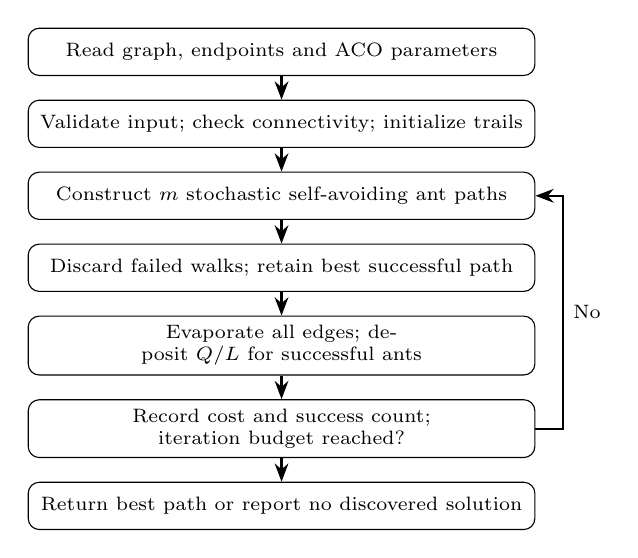
\begin{tikzpicture}[node distance=3mm, every node/.style={font=\scriptsize},box/.style={draw,rounded corners,align=center,text width=6.2cm,minimum height=6mm},arr/.style={-{Stealth},thick}]
\node[box] (a) {Read graph, endpoints and ACO parameters};
\node[box,below=of a] (b) {Validate input; check connectivity; initialize trails};
\node[box,below=of b] (c) {Construct $m$ stochastic self-avoiding ant paths};
\node[box,below=of c] (d) {Discard failed walks; retain best successful path};
\node[box,below=of d] (e) {Evaporate all edges; deposit $Q/L$ for successful ants};
\node[box,below=of e] (f) {Record cost and success count; iteration budget reached?};
\node[box,below=of f] (g) {Return best path or report no discovered solution};
\foreach \u/\v in {a/b,b/c,c/d,d/e,e/f,f/g} \draw[arr] (\u)--(\v);
\draw[arr] (f.east)--++(0.35,0)|-node[pos=0.25,right]{No}(c.east);
\end{tikzpicture}
\caption{ACO iteration flow. Disconnected endpoints and identical endpoints are handled before path construction.}
\label{fig:flow}
\end{figure}

\subsection{Algorithmic Procedure}
Algorithm~\ref{alg:aco} summarizes the implemented search.
\begin{algorithm}[tb]
\caption{ACO shortest-path search}\label{alg:aco}
\begin{algorithmic}[1]
\REQUIRE Positive weighted graph $G$, endpoints $s,t$, $m,T,\alpha,\beta,\rho,Q$
\ENSURE Best discovered path $P^*$ and cost $L^*$
\STATE Validate $G$, parameters and endpoints
\IF{$s=t$}
\STATE Return $[s]$ with cost zero
\ENDIF
\IF{$t$ is disconnected from $s$}
\STATE Return no path
\ENDIF
\STATE Set all trails to 1; $P^*\gets\emptyset$, $L^*\gets\infty$
\FOR{$r=1$ to $T$}
\STATE $S\gets\emptyset$
\FOR{$k=1$ to $m$}
\STATE Construct a self-avoiding walk using (2)
\IF{walk reaches $t$}
\STATE Add walk to $S$; update $P^*,L^*$ if improved
\ENDIF
\ENDFOR
\STATE Evaporate and reinforce trails using (3)--(5)
\STATE Record iteration statistics
\ENDFOR
\STATE Return $P^*,L^*$
\end{algorithmic}
\end{algorithm}

\subsection{Complexity and Baseline}
For $m$ ants, $T$ iterations and maximum degree $\Delta$, candidate evaluation takes $O(Tm|V|\Delta)$ time, while evaporation adds $O(T|E|)$. Storing the current population of successful paths uses $O(m|V|)$ auxiliary space, trails and adjacency lists use $O(|V|+|E|)$, and history uses $O(T)$. The initial connectivity check costs $O(|V|+|E|)$. Dijkstra's algorithm \cite{dijkstra1959added} provides an independent exact solution on these positive-weight graphs. Its heap-based implementation has $O((|V|+|E|)\log |V|)$ time complexity. Neither the baseline path nor its distances guide the ants.

\section{Implementation}
\subsection{Software Architecture}
The application is written in Python using the standard library, with Tkinter for the desktop interface. It runs from the Visual Studio Code terminal using \texttt{python app.py}; no third-party Python packages are needed. The \texttt{aco.py} module defines graph construction, input validation, the ant-colony solver and the Dijkstra baseline. The \texttt{app.py} module handles visualization and interaction. Reproducible evaluation is isolated in \texttt{experiments.py}, while \texttt{test\_aco.py} contains automated correctness checks.

\begin{figure}[tb]
\centering
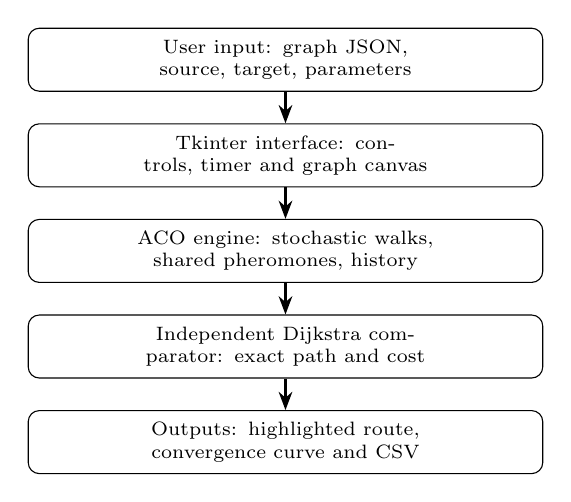
\begin{tikzpicture}[node distance=4mm,box/.style={draw,rounded corners,align=center,text width=6.3cm,minimum height=8mm,font=\scriptsize},arr/.style={-{Stealth},thick}]
\node[box] (a) {User input: graph JSON, source, target, parameters};
\node[box,below=of a] (b) {Tkinter interface: controls, timer and graph canvas};
\node[box,below=of b] (c) {ACO engine: stochastic walks, shared pheromones, history};
\node[box,below=of c] (d) {Independent Dijkstra comparator: exact path and cost};
\node[box,below=of d] (e) {Outputs: highlighted route, convergence curve and CSV};
\foreach \u/\v in {a/b,b/c,c/d,d/e} \draw[arr] (\u)--(\v);
\end{tikzpicture}
\caption{Software components and displayed outputs. The Dijkstra comparator evaluates the same graph independently; it does not feed path information into ACO.}
\label{fig:architecture}
\end{figure}

\subsection{Interface and Input Handling}
The interface supports a fixed demonstration network, a reproducible random network, and user-supplied JSON edge lists. Users choose source, destination, colony size, iteration count, $\alpha$, $\beta$, evaporation and solver seed. The deposit constant is $Q=10$. Each timer callback performs one colony iteration, redraws pheromone thickness and the current best route, and updates the convergence graph. Pause/resume and restart are supported, and iteration statistics can be exported as CSV. The GUI random preset has 16 nodes; the evaluation graphs described below are generated separately by the experiment script.

Input validation rejects nonpositive or nonfinite weights, self-loops, invalid parameters and missing endpoints. Graphs must be undirected. Isolated vertices are supported. If $s=t$, the result is the singleton path with cost zero. A graph traversal identifies unreachable destinations. On a reachable graph, exhausting the stochastic search without a solution is distinguished from proving that no route exists.

\begin{table}[tb]
\caption{Default Evaluation Configuration}
\label{tab:parameters}
\centering
\begin{tabular}{lc}\hline
Parameter & Value\\\hline
Ants per iteration $m$ & 40\\
Iterations $T$ & 100\\
Pheromone exponent $\alpha$ & 1\\
Heuristic exponent $\beta$ & 2\\
Evaporation $\rho$ & 0.3\\
Deposit constant $Q$ & 10\\
Initial trail / numerical floor & $1$ / $10^{-12}$\\
Solver seeds per graph & 0--19\\
Random graph seed & 42\\\hline
\end{tabular}
\end{table}

\subsection{Demonstration Network}
Figure~\ref{fig:graph} contains all 13 edges of the eight-node demo. Its optimum is $A\!\to\!B\!\to\!C\!\to\!D\!\to\!E\!\to\!F\!\to\!G\!\to\!H$, with cost $2+1+1+2+1+2+1=10$. The diagram is generated from the same edge list used by the program; edge costs are not Euclidean distances.

\begin{figure}[tb]
\centering
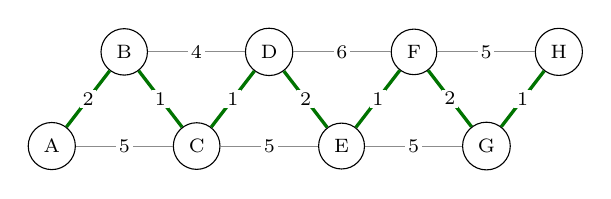
\begin{tikzpicture}[scale=0.92, every node/.style={font=\scriptsize},v/.style={circle,draw,fill=white,minimum size=5mm},e/.style={draw=black!45},best/.style={draw=green!45!black,very thick}]
\foreach \n/\x/\y in {A/0/0,B/1/1.3,C/2/0,D/3/1.3,E/4/0,F/5/1.3,G/6/0,H/7/1.3} \node[v] (\n) at (\x,\y) {\n};
\foreach \a/\b/\w in {A/B/2,B/C/1,C/D/1,D/E/2,E/F/1,F/G/2,G/H/1} \draw[best] (\a)--node[fill=white,inner sep=1pt]{\w}(\b);
\foreach \a/\b/\w in {A/C/5,B/D/4,C/E/5,D/F/6,E/G/5,F/H/5} \draw[e] (\a)--node[fill=white,inner sep=1pt]{\w}(\b);
\end{tikzpicture}
\caption{Weighted demo network. Green edges identify the exact optimum of cost 10. Grey edges remain valid alternatives explored by ants.}
\label{fig:graph}
\end{figure}

\section{Results and Discussion}
\subsection{Experimental Protocol}
Four fixed graphs were evaluated: the eight-node demo and three random graphs with 15, 30 and 50 vertices. Each random graph begins with a chain connecting consecutive labels; every remaining unordered pair is then added independently with probability 0.18. Integer weights are sampled uniformly from 1 to 20. Each graph uses generator seed 42, and queries run from vertex 0 to vertex $n-1$. Thus all evaluation graphs are connected. Each graph was evaluated with 20 solver seeds (0--19), using Table~\ref{tab:parameters}. These are repeated solver trials on four graph instances, not 80 independent graph instances.

Runtime uses Python's monotonic performance counter. ACO timing covers the 100-iteration search after solver initialization; it excludes graph construction, GUI drawing and exports. Dijkstra runtime is the mean of 100 direct calls on the same graph. Timing measurements are descriptive and machine-dependent, and do not establish a general performance bound. The delivered CSV stores every seed's route, cost, runtime and first iteration reaching the exact optimum. The environment was Python 3.13.2 on Windows.

For a returned solution, the relative cost gap is
\begin{equation}
\mathrm{Gap}(\%)=100\frac{L_{\mathrm{ACO}}-L_{\mathrm{Dijkstra}}}{L_{\mathrm{Dijkstra}}}.
\end{equation}
The optimal-hit count is the number of runs matching the exact baseline cost. Mean gaps below are calculated over runs that returned a path; failures, if present, are counted separately in the found column.

\begin{table}[tb]
\caption{Measured Outcomes Across 20 Solver Seeds}
\label{tab:results}
\centering\scriptsize
\begin{tabular}{lrrrrrr}\hline
Graph & $|V|$ & $|E|$ & Opt. & Found & Hits & Gap (\%)\\\hline
Demo & 8 & 13 & 10 & 20/20 & 20/20 & 0.00 \\
Random-15 & 15 & 30 & 11 & 20/20 & 20/20 & 0.00 \\
Random-30 & 30 & 106 & 16 & 20/20 & 20/20 & 0.00 \\
Random-50 & 50 & 250 & 3 & 20/20 & 20/20 & 0.00 \\
\hline\end{tabular}
\end{table}
\begin{table}[tb]
\caption{Measured Search Time (Milliseconds)}
\centering\small
\begin{tabular}{lrr}\hline
Graph & ACO mean $\pm$ sample SD & Dijkstra mean\\\hline
Demo & $406.29 \pm 95.77$ & 0.0302 \\
Random-15 & $366.69 \pm 88.43$ & 0.0245 \\
Random-30 & $1409.05 \pm 271.35$ & 0.1191 \\
Random-50 & $216.33 \pm 11.24$ & 0.0216 \\
\hline\end{tabular}\end{table}

For Demo, ACO returned a feasible path in 20 of 20 runs and matched the exact cost 10 in 20 runs; the maximum observed cost gap was 0.00\%. For Random-15, ACO returned a feasible path in 20 of 20 runs and matched the exact cost 11 in 20 runs; the maximum observed cost gap was 0.00\%. For Random-30, ACO returned a feasible path in 20 of 20 runs and matched the exact cost 16 in 20 runs; the maximum observed cost gap was 0.00\%. For Random-50, ACO returned a feasible path in 20 of 20 runs and matched the exact cost 3 in 20 runs; the maximum observed cost gap was 0.00\%. These observations are specific to the tested instances and seeds, and do not imply an optimality guarantee.

\subsection{Convergence and Runtime}
Figure~\ref{fig:convergence} reports recorded best-so-far costs for solver seed 0. In all four seed-0 runs, the optimum was already found in the first iteration, so these particular curves are flat; they do not demonstrate gradual convergence. The curve is monotone because the implementation retains its incumbent solution; this property alone does not prove that the optimum has been found. Figures~\ref{fig:hits} and \ref{fig:runtime} summarize the repeated-run outcomes. ACO performs thousands of stochastic path constructions, whereas the exact baseline solves one static query directly. For this task, Dijkstra is the practical exact reference; the value of the project is an observable implementation of collective stochastic search.

\begin{figure}[tb]\centering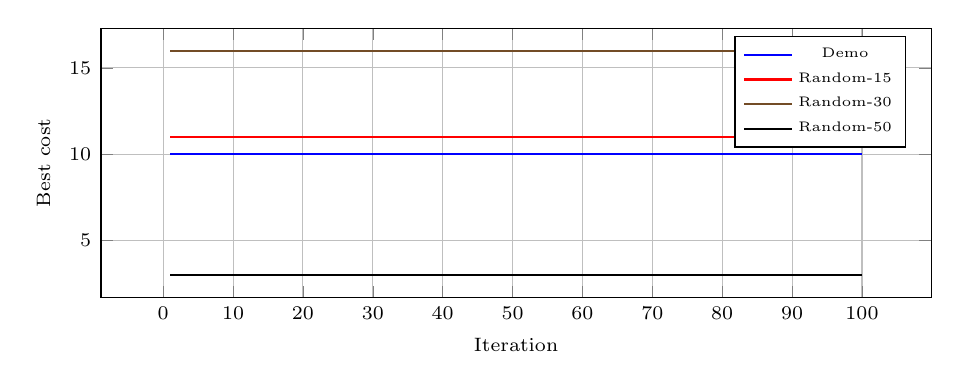
\begin{tikzpicture}\begin{axis}[width=\columnwidth,height=5cm,tick label style={font=\scriptsize},label style={font=\scriptsize},legend style={font=\tiny},xlabel={Iteration},ylabel={Best cost},legend pos=north east,grid=major]
\addplot+[no marks,thick] coordinates {(1,10.0) (2,10.0) (3,10.0) (4,10.0) (5,10.0) (6,10.0) (7,10.0) (8,10.0) (9,10.0) (10,10.0) (11,10.0) (12,10.0) (13,10.0) (14,10.0) (15,10.0) (16,10.0) (17,10.0) (18,10.0) (19,10.0) (20,10.0) (21,10.0) (22,10.0) (23,10.0) (24,10.0) (25,10.0) (26,10.0) (27,10.0) (28,10.0) (29,10.0) (30,10.0) (31,10.0) (32,10.0) (33,10.0) (34,10.0) (35,10.0) (36,10.0) (37,10.0) (38,10.0) (39,10.0) (40,10.0) (41,10.0) (42,10.0) (43,10.0) (44,10.0) (45,10.0) (46,10.0) (47,10.0) (48,10.0) (49,10.0) (50,10.0) (51,10.0) (52,10.0) (53,10.0) (54,10.0) (55,10.0) (56,10.0) (57,10.0) (58,10.0) (59,10.0) (60,10.0) (61,10.0) (62,10.0) (63,10.0) (64,10.0) (65,10.0) (66,10.0) (67,10.0) (68,10.0) (69,10.0) (70,10.0) (71,10.0) (72,10.0) (73,10.0) (74,10.0) (75,10.0) (76,10.0) (77,10.0) (78,10.0) (79,10.0) (80,10.0) (81,10.0) (82,10.0) (83,10.0) (84,10.0) (85,10.0) (86,10.0) (87,10.0) (88,10.0) (89,10.0) (90,10.0) (91,10.0) (92,10.0) (93,10.0) (94,10.0) (95,10.0) (96,10.0) (97,10.0) (98,10.0) (99,10.0) (100,10.0)};\addlegendentry{Demo}
\addplot+[no marks,thick] coordinates {(1,11.0) (2,11.0) (3,11.0) (4,11.0) (5,11.0) (6,11.0) (7,11.0) (8,11.0) (9,11.0) (10,11.0) (11,11.0) (12,11.0) (13,11.0) (14,11.0) (15,11.0) (16,11.0) (17,11.0) (18,11.0) (19,11.0) (20,11.0) (21,11.0) (22,11.0) (23,11.0) (24,11.0) (25,11.0) (26,11.0) (27,11.0) (28,11.0) (29,11.0) (30,11.0) (31,11.0) (32,11.0) (33,11.0) (34,11.0) (35,11.0) (36,11.0) (37,11.0) (38,11.0) (39,11.0) (40,11.0) (41,11.0) (42,11.0) (43,11.0) (44,11.0) (45,11.0) (46,11.0) (47,11.0) (48,11.0) (49,11.0) (50,11.0) (51,11.0) (52,11.0) (53,11.0) (54,11.0) (55,11.0) (56,11.0) (57,11.0) (58,11.0) (59,11.0) (60,11.0) (61,11.0) (62,11.0) (63,11.0) (64,11.0) (65,11.0) (66,11.0) (67,11.0) (68,11.0) (69,11.0) (70,11.0) (71,11.0) (72,11.0) (73,11.0) (74,11.0) (75,11.0) (76,11.0) (77,11.0) (78,11.0) (79,11.0) (80,11.0) (81,11.0) (82,11.0) (83,11.0) (84,11.0) (85,11.0) (86,11.0) (87,11.0) (88,11.0) (89,11.0) (90,11.0) (91,11.0) (92,11.0) (93,11.0) (94,11.0) (95,11.0) (96,11.0) (97,11.0) (98,11.0) (99,11.0) (100,11.0)};\addlegendentry{Random-15}
\addplot+[no marks,thick] coordinates {(1,16.0) (2,16.0) (3,16.0) (4,16.0) (5,16.0) (6,16.0) (7,16.0) (8,16.0) (9,16.0) (10,16.0) (11,16.0) (12,16.0) (13,16.0) (14,16.0) (15,16.0) (16,16.0) (17,16.0) (18,16.0) (19,16.0) (20,16.0) (21,16.0) (22,16.0) (23,16.0) (24,16.0) (25,16.0) (26,16.0) (27,16.0) (28,16.0) (29,16.0) (30,16.0) (31,16.0) (32,16.0) (33,16.0) (34,16.0) (35,16.0) (36,16.0) (37,16.0) (38,16.0) (39,16.0) (40,16.0) (41,16.0) (42,16.0) (43,16.0) (44,16.0) (45,16.0) (46,16.0) (47,16.0) (48,16.0) (49,16.0) (50,16.0) (51,16.0) (52,16.0) (53,16.0) (54,16.0) (55,16.0) (56,16.0) (57,16.0) (58,16.0) (59,16.0) (60,16.0) (61,16.0) (62,16.0) (63,16.0) (64,16.0) (65,16.0) (66,16.0) (67,16.0) (68,16.0) (69,16.0) (70,16.0) (71,16.0) (72,16.0) (73,16.0) (74,16.0) (75,16.0) (76,16.0) (77,16.0) (78,16.0) (79,16.0) (80,16.0) (81,16.0) (82,16.0) (83,16.0) (84,16.0) (85,16.0) (86,16.0) (87,16.0) (88,16.0) (89,16.0) (90,16.0) (91,16.0) (92,16.0) (93,16.0) (94,16.0) (95,16.0) (96,16.0) (97,16.0) (98,16.0) (99,16.0) (100,16.0)};\addlegendentry{Random-30}
\addplot+[no marks,thick] coordinates {(1,3.0) (2,3.0) (3,3.0) (4,3.0) (5,3.0) (6,3.0) (7,3.0) (8,3.0) (9,3.0) (10,3.0) (11,3.0) (12,3.0) (13,3.0) (14,3.0) (15,3.0) (16,3.0) (17,3.0) (18,3.0) (19,3.0) (20,3.0) (21,3.0) (22,3.0) (23,3.0) (24,3.0) (25,3.0) (26,3.0) (27,3.0) (28,3.0) (29,3.0) (30,3.0) (31,3.0) (32,3.0) (33,3.0) (34,3.0) (35,3.0) (36,3.0) (37,3.0) (38,3.0) (39,3.0) (40,3.0) (41,3.0) (42,3.0) (43,3.0) (44,3.0) (45,3.0) (46,3.0) (47,3.0) (48,3.0) (49,3.0) (50,3.0) (51,3.0) (52,3.0) (53,3.0) (54,3.0) (55,3.0) (56,3.0) (57,3.0) (58,3.0) (59,3.0) (60,3.0) (61,3.0) (62,3.0) (63,3.0) (64,3.0) (65,3.0) (66,3.0) (67,3.0) (68,3.0) (69,3.0) (70,3.0) (71,3.0) (72,3.0) (73,3.0) (74,3.0) (75,3.0) (76,3.0) (77,3.0) (78,3.0) (79,3.0) (80,3.0) (81,3.0) (82,3.0) (83,3.0) (84,3.0) (85,3.0) (86,3.0) (87,3.0) (88,3.0) (89,3.0) (90,3.0) (91,3.0) (92,3.0) (93,3.0) (94,3.0) (95,3.0) (96,3.0) (97,3.0) (98,3.0) (99,3.0) (100,3.0)};\addlegendentry{Random-50}
\end{axis}\end{tikzpicture}\caption{Recorded seed-0 convergence on each fixed evaluation graph.}\label{fig:convergence}\end{figure}

\begin{figure}[tb]\centering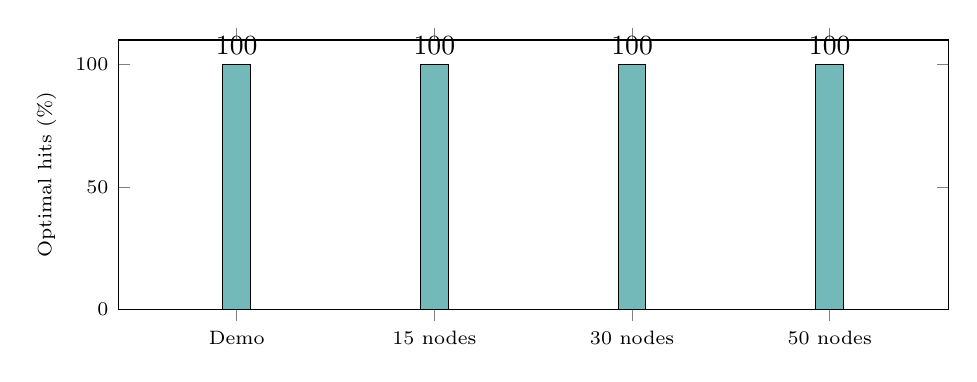
\begin{tikzpicture}\begin{axis}[width=\columnwidth,height=5cm,tick label style={font=\scriptsize},label style={font=\scriptsize},legend style={font=\tiny},ybar,ymin=0,ymax=110,xmin=-0.6,xmax=3.6,xtick={0,1,2,3},xticklabels={Demo,15 nodes,30 nodes,50 nodes},ylabel={Optimal hits (\%)},nodes near coords]
\addplot[fill=teal!55] coordinates {(0,100) (1,100) (2,100) (3,100)};\end{axis}\end{tikzpicture}\caption{Fraction of 20 solver seeds matching Dijkstra on each fixed graph.}\label{fig:hits}\end{figure}

\begin{figure}[tb]\centering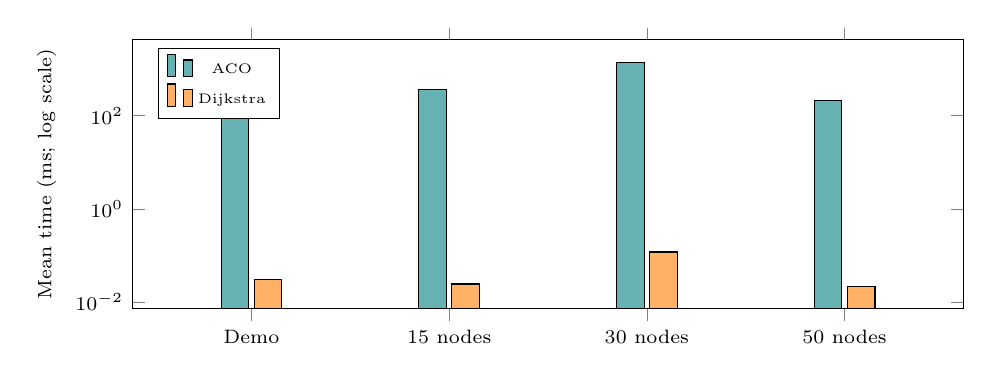
\begin{tikzpicture}\begin{axis}[width=\columnwidth,height=5cm,tick label style={font=\scriptsize},label style={font=\scriptsize},legend style={font=\tiny},ybar,ymode=log,log origin=infty,xmin=-0.6,xmax=3.6,xtick={0,1,2,3},xticklabels={Demo,15 nodes,30 nodes,50 nodes},ylabel={Mean time (ms; log scale)},legend pos=north west]
\addplot[fill=teal!60] coordinates {(0,406.288975) (1,366.694685) (2,1409.053345) (3,216.330440)};
\addplot[fill=orange!60] coordinates {(0,0.030238) (1,0.024501) (2,0.119104) (3,0.021634)};
\legend{ACO,Dijkstra}\end{axis}\end{tikzpicture}\caption{Measured search runtimes. ACO averages 20 runs; Dijkstra averages 100 calls. Initialization and GUI time are excluded from ACO.}\label{fig:runtime}\end{figure}

\subsection{Verification and Limitations}
Eight automated tests passed: the known demo optimum and route validity; disconnected endpoints; identical endpoints; fixed-seed reproducibility; invalid inputs; the single-edge evaporation/deposit calculation; a graph containing a dead end; and comparison of valid stochastic solutions against exact costs on five additional small random graphs. A separate GUI smoke check exercised construction, run, pause, resume and reset.

The study is limited to small static graphs, one parameter configuration and one graph instance per random size. The 15-node generated instance has a direct source--target edge on its optimum and should not be interpreted as a difficult general benchmark. Different graph structures and parameter settings can yield worse costs, failures or premature convergence. Ants that enter dead ends are discarded, so sparse branching networks can waste trials. No sensitivity analysis, dynamic-edge experiment, A* comparison or real-world robotic evaluation was performed. Claims about dynamic environments in the background sections are motivation rather than findings established by these experiments.

\section{Conclusion}
A runnable Python application was implemented for shortest-path search using Ant Colony Optimization. The system combines stochastic self-avoiding walks, inverse-cost heuristics, evaporation and successful-path reinforcement, with interactive graph visualization and exportable experiment records. An independent Dijkstra solver makes solution quality directly checkable. The reported experiments quantify actual outcomes on four fixed positive-weight graphs and show the computational overhead of repeated ant exploration relative to an exact static-graph method. The implementation is therefore useful for demonstrating ACO mechanisms, while finite-run optimality remains unguaranteed. Future work can evaluate multiple graph instances per size, parameter sensitivity, dynamic edge changes, and more effective recovery from dead ends under a clearly specified benchmark protocol.


\begin{thebibliography}{00}

\bibitem{dorigo1996}
M. Dorigo, V. Maniezzo, and A. Colorni,
``Ant System: Optimization by a Colony of Cooperating Agents,''
\textit{IEEE Transactions on Systems, Man, and Cybernetics--Part B},
vol. 26, no. 1, pp. 29--41, 1996.

\bibitem{dorigo1997}
M. Dorigo and L. M. Gambardella,
``Ant Colony System: A Cooperative Learning Approach to the Traveling Salesman Problem,''
\textit{IEEE Transactions on Evolutionary Computation},
vol. 1, no. 1, pp. 53--66, 1997.

\bibitem{shortestpathaco}
A. Colorni, M. Dorigo, and V. Maniezzo,
``Distributed Optimization by Ant Colonies,''
in \textit{Proceedings of the First European Conference on Artificial Life},
Paris, France, pp. 134--142, 1991.


\bibitem{ieaco2025}
P. Li et al.,
``An Intelligently Enhanced Ant Colony Optimization Algorithm for Global Path Planning of Mobile Robots,''
\textit{Sensors},
vol. 25, no. 5, 2025.

\bibitem{itaco2025}
J. Ma et al.,
``Improved Trimming Ant Colony Optimization Algorithm for Mobile Robot Path Planning,''
\textit{Algorithms},
vol. 18, no. 5, 2025.

\bibitem{msgaco2025}
Z. Li et al.,
``Research on Robot Path Planning Based on Multi-Strategy Improved Ant Colony Algorithm,''
\textit{Information Sciences},
2025.

\bibitem{iqaco2025}
D. Li et al.,
``Research on Mobile Robot Path Planning Based on Improved Q-Evaluation Ant Colony Optimization Algorithm,''
\textit{Engineering Applications of Artificial Intelligence},
2025.

\bibitem{deliveryaco2025}
L. Huang et al.,
``Path Planning for Delivery Robots Based on an Improved Ant Colony Optimization Algorithm,''
\textit{Sensors},
2025.

\bibitem{robotaco2025}
G. Shi et al.,
``Improved Ant Colony Algorithm-Based Path Planning for Mobile Robots,''
\textit{Proceedings of SPIE},
2025.

\bibitem{adaptiveaco2025}
J. Cui et al.,
``Multi-Strategy Adaptable Ant Colony Optimization Algorithm for Path Planning,''
\textit{Expert Systems with Applications},
2024.

\bibitem{mseaco2026}
Y. Zhuo et al.,
``Path Planning for Mobile Robots Based on Multi-Strategy Enhanced Ant Colony Optimization Algorithm,''
\textit{International Journal of Computational Intelligence Systems},
2026.

\bibitem{enhancedaco2026}
L. Yu et al.,
``An Enhanced Ant Colony Optimization Algorithm for Path Planning of a Mobile Robot,''
\textit{Optimal Control Applications and Methods},
2026.

\bibitem{pfaco2026}
Y. Liu et al.,
``Pheromone-Focused Ant Colony Optimization Algorithm for Path Planning,''
2026.

\bibitem{idlaco2026}
X. Zeng et al.,
``I-DL-ACO: Double Layer Ant Colony Optimization for Robot Navigation Path Planning,''
\textit{Robotics and Autonomous Systems},
2026.

\bibitem{dijkstra1959added}
E. W. Dijkstra, ``A Note on Two Problems in Connexion with Graphs,''
\textit{Numerische Mathematik}, vol. 1, pp. 269--271, 1959,
doi: 10.1007/BF01386390.

\end{thebibliography}

\end{document}